\chapter{The Standard Model and Beyond} \label{chap:standard_model}

The Standard Model (SM) of Particle Physics is humanities best "guess" at the
force laws that describe the observed behavior of all particles in our
universe. Its formulation is a collection of Quantum Field Theories (QFT) that
describe the following interactions of elementary matter in Nature: the
electromagnetic force, the weak nuclear force and the strong nuclear force.
Gravity is noticeably absent as currently there is no viable quantum theory for
observed gravitational effects.  The Glashow-Weinberg-Salam theory of Quantum
Electrodynamics (QED) describes the electromagnetic and weak forces, while
Quantum Chromodyanmics (QCD) describes the strong force.  These theories form
the following symmetry group of the Standard Model.

\begin{equation} \label{eq:standardmodel:symmetry_group}
  \underbrace{\text{SU}_\text{C}(3)}_\text{QCD} \otimes \underbrace{\text{SU}_\text{L}(2) \otimes \text{U}_\text{Y}(1)}_\text{QED}.
\end{equation}

The gauge principle states that the SM Lagrangian and its predictions must be
invariant under local transformations using an operator from any of these
constituent groups.  Thus, any theory must only include transformations and
terms that maintain the local invariance of the complete Lagrangian.  In
particular, this requirement was violated by any attempt to include an explicit
mass term for the Gauge Bososns of QED and for all fermions.  Around 1960 a
possible solution to this lack of mass was proposed in the form of the
spontaneous breaking of the ElectroWeak symmetry, now known as the Higgs
mechanism.  In the following sections I will go into more detail about the
Lagrangian formalism of the Standard Model, QCD, QED and this recently verified
Higgs Mechanism.

\section{The Standard Model} \label{sec:theory:standardmodel}

At the turn of the 20th century, humanities understanding of the constituent
matter of the universe was limited to what could be seen with microscopes and
implied from the observations of light and electricity, giving evidence for
both the photon and the electron.  In the first half of the century the field
of subatomic physics was discovered with Rutherfords 1911 gold foil scattering
experiment \cite{Rutherford:1911zz} followed by the observation of
the wave-particle duality of nature with Compton's scattering experiment in
1923 \cite{PhysRev.21.483}. These were the first steps towards a Quantum Field
Theory representation of nature.  In the second half of the century experiments
delved deeper to discover that the nucleus contained structure thus the SM was
extended to include the complex mechanics of quarks and gluons
\cite{Fritzsch:1972jv}.  With the discovery of the Higgs in 2012, the Standard
Model has become even more firmly established as can be seen in the high level
of agreement between theory and experiment in \Cref{fig:xsection_measurements}.

\begin{figure}[!htbp]
  \begin{center}
    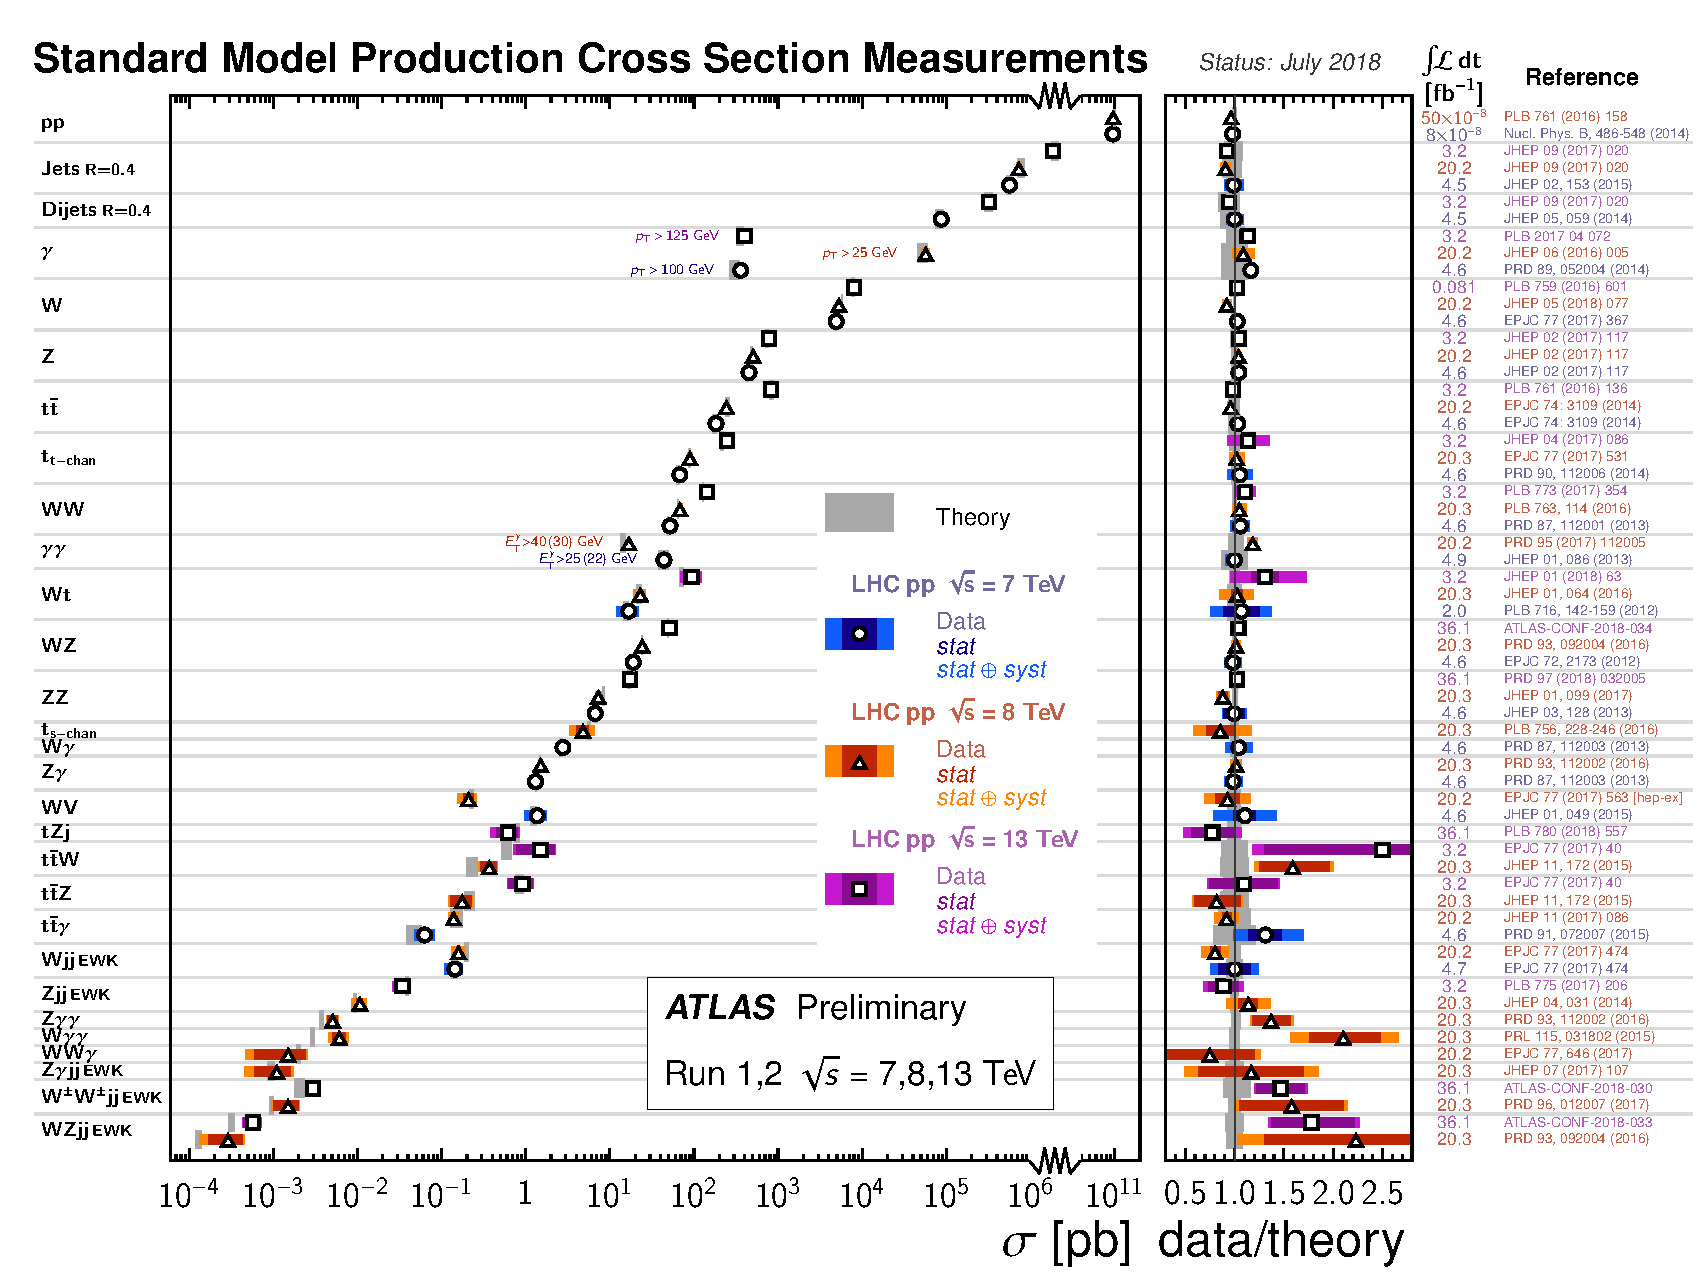
\includegraphics[width=\linewidth]{figures/theory/xsection_measurements.pdf}
\caption{ Summary of several Standard Model total and fiducial production cross
section measurements, corrected for leptonic branching fractions, compared to
the corresponding theoretical expectations \cite{StandardModelPublicResults}.
All theoretical expectations were calculated at NLO or higher. The dark-color
error bar represents the statistical uncertainty. The lighter-color error bar
represents the full uncertainty, including systematics and luminosity
uncertainties. The data/theory ratio, luminosity used and reference for each
measurement are also shown. Uncertainties for the theoretical predictions are
quoted from the original ATLAS papers. They were not always evaluated using the
same prescriptions for PDFs and scales.}
    \label{fig:xsection_measurements}
  \end{center}
\end{figure}

The QCD and GSW theories predict two classes of particles - fermions and bosons -
shown in \Cref{fig:standard_model}. These particles represent the quanta
of the quantum fields of the Standard Model and the mediators of the fundamental
forces of Nature.

\begin{figure}[!htbp]
  \begin{center}
    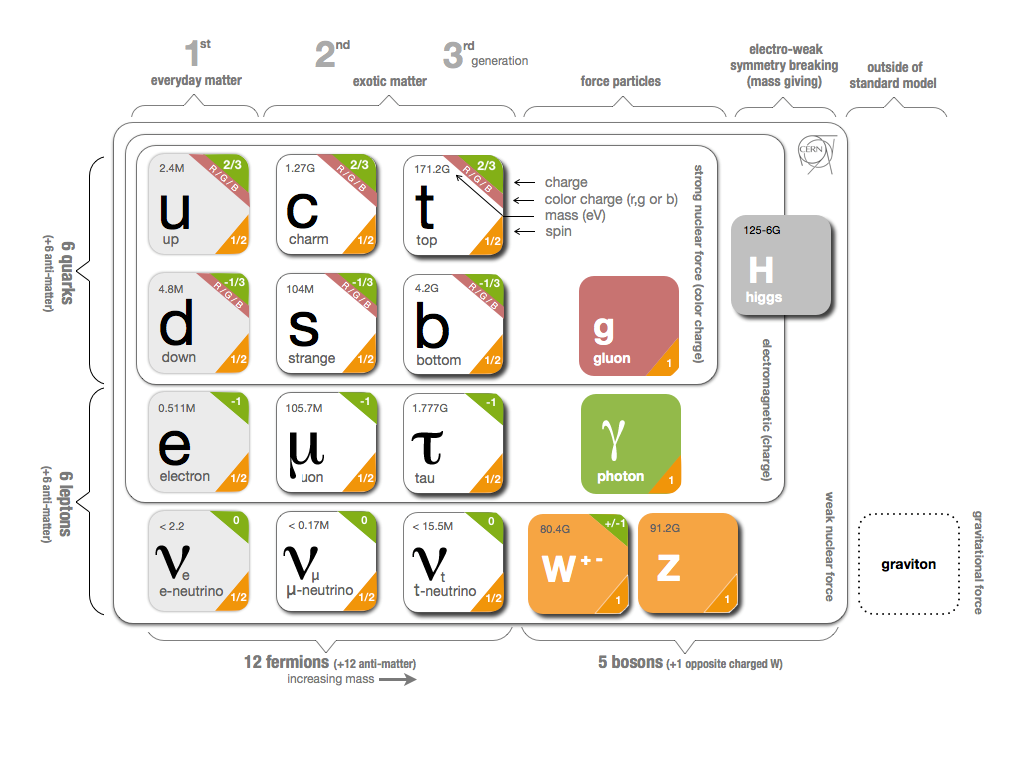
\includegraphics[width=\linewidth]{figures/theory/standard_model.png}
    \caption{ Table of all observed fundamental particles of the Standard
Model. \cite{Purcell:1473657}}
    \label{fig:standard_model}
  \end{center}
\end{figure}

\subsection{Bosons} \label{sec:theory:bosons}

The spin-1 particles are known as the vector gauge bosons and are the force
carriers of the SM.  The most commonly known is the electromagnetic force's
uncharged and massless photon ($\gamma$) which interacts with all particles
charged under $U(1)_{\text{em}}$ and is often referred to as ``light."  The
weak nuclear force is involved in nuclear interactions such as beta decays and
is carried by 3 bosons, all of which have mass and couple to fermions.  The
$W^{\pm}$ bosons mediate the charged weak interaction and allow for flavor
changing currents, while the $Z$ boson mediates the neutral weak interaction.
Finally there are 8 massless gluons which mediate the strong force and only
interact with fermions that have a ``color" charge such as the quarks contained
inside the nucleons. The only spin-0 boson, the Higgs Boson ($H$) is the key to
generating mass terms in the SM Lagrangian for the massive gauge bosons and for
fermions.  This is done through the so-called Higgs mechanism
\cite{Thomson:2013zua} and is discussed in more detail in
\Cref{sec:theory:higgs}.

\subsection{Fermions} \label{sec:theory:fermions}

The spin-1/2 particles can be further broken up into two distinct families of
particles, the leptons and the quarks, both of which contain three
``generations" each with an ``up"- and ``down"-type particle where ``up" and
``down" differentiate the two components of the weak isospin doublet.  The
``down"-type leptons are the electrically charged electron ($e$), muon ($\mu$)
and tau ($\tau$) while the ``up"-type are their electrically neutral
counterparts $\nu_e$, $\nu_\mu$, $\nu_\tau$. The ``up"-type quarks are the up
($u$), charm ($c$), and top ($t$), each with a $+2/3$ electric charge, while
the ``down"-type quarks are the down ($d$), strange ($s$), and bottom ($b$),
all of which have a $-1/3$ electric charge.  Each quark carries a ``color"
charge thus allowing them to couple to gluons and  participate in strong force
interactions.  Due to the observed color confinement of the strong force these
quarks are only observed in colorless bound states known as ``mesons" (1 quark
and 1 anti-quark) and ``baryons" (3 quarks or anti-quarks).  All of the above
fermions have an anti-particle partner with the opposite weak isospin.


Quantum Chromodynamics is the continuation of the mathematical framework
established by the electroweak formalism in (\Cref{sec:theory:gsw}, this time
for the strong force described by the $SU(3)_C$ gauge group, where $C$
represents the ``color" charge of QCD \cite{Campbell:2017hsr}.  This
color charge doesn't imply actual visible color, but is useful as an analogy to
the visible spectrum where a combination of red, green, and blue generates
white.  For QCD the combination of red, green, and blue color charges can
result in a colorless object.  As mentioned in \Cref{sec:theory:fermions}, the
quarks have a color (anti-color) charge defining color triplet field which
transforms under the general $SU(3)$ transformation as

\begin{equation}
q = \left( \begin{matrix} q_{r} \\ q_{g} \\ q_{b} \end{matrix} \right)
\rightarrow q^{'} = exp \left( ig_{s} \sum_{k=1}^{8} \eta_{k}(x)
\frac{\lambda_k}{2} \right) q
\end{equation}

Here the $\lambda_{k}$ are the Gell-Mann generators for $SU(3)$, $\eta(x)_{k}$ is the
space-time dependency for each generator, and  $g_s$ is the strong coupling constant.
As with the electroweak Lagrangian, the introduction of these space-time dependent terms adds new
terms into the kinematic portion of the Lagrangian and spoils the gauge 
invariance.  Again, a covariant derivative is introduced 

\begin{equation}
D_{\mu} = \partial_{\mu} - ig_{s}G_{\mu}^{k}\frac{\lambda_{k}}{2}
\end{equation}

to restore gauge invariance. The $G_{\mu}^{k}$ are the new fields introduced
for the 8 gluons.  These new fields transform under $SU(3)$ as

\begin{equation} \label{eq:qcd:gluon_field}
G_{\mu}^{k} \rightarrow G_{\mu}^{'k} = G_{\mu}^{k} + \partial_{\mu}\eta_{k}(x) +
g_{s}f_{klm}\eta_{l}(x)G_{\mu}^{m}
\end{equation}

Given these definitions the QCD Lagrangian ($\mathcal{L}_{QCD}$) can be
constructed as 

\begin{equation} \label{eq:qcd:qcd_lagrangian}
\mathcal{L}_{QCD} = \bar{q}(i\gamma_{\mu}D^{\mu} - m_{q})q -
\frac{1}{4}G_{k}^{\mu\nu}G_{k\mu\nu}
\end{equation}

where the gluon field tensor $G_{k}^{\mu\nu}$ is defined as

\begin{equation} \label{eq:qcd:gluon_tensor}
G_{k}^{\mu\nu} = \partial^{\mu}G_{k}^{\nu} - \partial^{\nu}G_{k}^{\mu} +
g_{s}f_{klm}G_{\l}^{\mu}G_{m}^{\nu}.
\end{equation}

The strong force is peculiar in that experiments observe only colorless objects
in the form of bound states of quarks known as hadrons.  Qualitatively, the
potential between a bound state of quarks (meson or baryon) gets stronger with
separation, unlike the other forces.  At the point where the system would
separate into color-charged objects, it becomes energetically favorable to
produce a quark/anti-quark pair in a process known as hadronization.  In other
words, attempting to separate a bound quark state into its colored constituents
simply results in new colorless bound states.  This requirement of colorless
objects by the strong force is known as color confinement. For highly energetic
strong interactions at hadron colliders the result is an expanding chain of
hadronizing quarks and gluons and their decay products known as a jet.


\section{Quantum Electrodynamics} \label{sec:theory:qed}

In the SM the Electromagnetic and Weak nuclear forces are unified into the
Electroweak interaction which is represented by the $SU(2)_L \times U(1)_Y$
gauge group. The L represents the physical observable that the Weak interaction,
and thus the $SU(2)$ transformation, only acts on left handed particle states.
The Y states that this is the $U(1)$ symmetry for the weak hypercharge Y instead
of the electromagnetic charge.  The particle states for these interactions are
solutions to the Dirac equation and are represented as Dirac spinor doublets
($\boldsymbol{\Psi_L}$) for the left handed states, and as Dirac spinor singlets
($\Psi_R$) for the right handed states.  Thus when a general transformation from
the Electroweak gague group is applied to the left handed spinor doublet you get
\Cref{eq:qed:doublet}

\begin{equation} \label{eq:qed:doublet} 
\boldsymbol{\Psi_L} \rightarrow \boldsymbol{\Psi_L}^{'} = exp \left(
\underbrace{ ig^{'} \frac{Y_L}{2}
\zeta (x) }_{U(1)_Y} + \underbrace{ ig_{W} \boldsymbol{\alpha}(x) \cdot
\text{\bf{T}} }_{SU(2)_L} \right) \boldsymbol{\Psi_L}.
\end{equation}

For the right handed spinor singlet the $SU(2)_L$ doesn't contribute and
you get \Cref{eq:qed:singlet}

\begin{equation} \label{eq:qed:singlet} 
{\Psi_R} \rightarrow \Psi_R^{'} = exp \left( \underbrace{ ig^{'} \frac{Y_R}{2}
\zeta (x) }_{U(1)_Y} \right) \Psi_R.
\end{equation}

We can see that these local gauge transformations have introduced space-time
dependant terms $\boldsymbol{\alpha}(x)$ and $\zeta(x)$ into our electroweak
Lagrangian.  Due to the derivatives contained within the kinetic term of this
lagrangian, this new configuration would introduce additional terms, thus
violating our required local gauge invariance.  Luckily, we can remove these
additional terms by replacing the standard derivative ($\partial_{\mu}$) with th
covariant derivative ($D_{\mu}$) as seen in \Cref{eq:qed:left} for the
left handed states and \Cref{eq:qed:right} for the right handed states.

\begin{align} 
\label{eq:qed:left} 
D_\mu &= \partial_{\mu}
- \underbrace{\frac{1}{2}ig^{'}B_{\mu}Y_{L}}_{U(1)_Y} -
  \underbrace{\frac{1}{2}ig_{W}\bf{W}_\mu \cdot \boldsymbol{\tau}}_{SU(2)_L} \\
\label{eq:qed:right} 
D_\mu &= \partial_{\mu}  - \underbrace{\frac{1}{2}ig^{'}B_{\mu}Y_{R}}_{U(1)_Y} 
\end{align}

Here we see two new gauge fields; $B_\mu$ the weak hypercharge field and
$\boldsymbol{W_\mu}$ the charged weak field as well as the associated coupling
constants $g^{'}, g_{W}, Y_{L}, Y_{R}$ and the $SU(2)$ generators
$\boldsymbol{\tau}$.   Next we right down the transformation properies of these
new fields 

\begin{align}
\boldsymbol{W}_{\mu}(x) &\rightarrow \boldsymbol{W}_{\mu}^{'}(x) =
\boldsymbol{W}_{\mu} + \partial_{\mu} \boldsymbol{\alpha}(x) +
g_{W}\boldsymbol{W}_{\mu}(x) \times \boldsymbol{\alpha}(x)
\\ 
B_{\mu} &\rightarrow B_{\mu}^{'} = B_{\mu} +
\frac{1}{g^{'}}\partial_{\mu}\zeta(x)
\end{align}

The form of these fields is chosen such that the final Lagrangian is invariant
under $SU(2)_L \times U(1)_Y$ transformations, and thus we have restored gauge
invariance for the kinetic term of our electroweak Lagrangian!  Inserting these
new definitions into the Lagrangian for the spinor field $\Psi$ which satisfies
the free-particle Dirac equation we get

\begin{equation} \label{eq:qed:fermion_lagrangian}
\mathcal{L} = i\boldsymbol{\bar{\Psi}_L}\gamma^{\mu} \left( \partial_{\mu}
- \frac{1}{2}ig^{'}B_{\mu}Y_{L} - \frac{1}{2}ig_{W}\bf{W}_\mu \cdot
  \boldsymbol{\tau} \right) \boldsymbol{\Psi_L} + i \bar{\Phi}_{R}\gamma^{\mu}
\left(\partial_{\mu} - \frac{1}{2}ig^{'}B_{\mu}Y_{R} \right) \Phi_{R}
\end{equation}

Next we must construct the gauge field self interaction and mass terms

\begin{equation} \label{eq:qed:gauge_lagrangian}
\mathcal{L} = -\frac{1}{4}\boldsymbol{F}_{\mu\nu}\boldsymbol{F}^{\mu\nu}
-\frac{1}{4}B_{\mu\nu}B^{\mu\nu} +
\frac{1}{2}M_{W}^{2}\boldsymbol{W}_{\mu}\boldsymbol{W}^{\mu} +
\frac{1}{2}M_{B}^{2}B_{\mu}B^{\mu}
\end{equation}

where the field tensors $\boldsymbol{F}^{\mu\nu}$ and $B^{\mu\nu}$ are defined
to be

\begin{align}
\boldsymbol{F}^{\mu\nu}  &= \partial^{\mu}\boldsymbol{W}^{\nu} -
\partial^{\nu}\boldsymbol{W}^{\mu} + g\boldsymbol{W}^{\mu} \times
\boldsymbol{W}^{\nu} \\
B^{\mu\nu} &=  \partial^{\mu}\boldsymbol{B}^{\nu} -
\partial^{\nu}\boldsymbol{B}^{\mu}
\end{align}

The field tensor terms in \Cref{eq:qed:gauge_lagrangian} are invariant
under our gauge transformations, but simply plugging in
\Cref{eq:qed:left} or \Cref{eq:qed:right} into the mass terms shows that
these terms violate gauge invariance thus implying $M_{W} = 0$ and $M_{B} = 0$
in direct contradiction of the observed masses of the weak gauge bosons.  This
issue arises again for fermion mass terms as illustrated below for the elctron
field ($e$) expanded in its chiral basis.

\begin{equation}
m_{e}\bar{e}e = m_{e} \left( \begin{matrix}e^{\dagger}_{R} &
e^{\dagger}_{L} \end{matrix} \right) \left( \begin{matrix} e_{L}
\\ e_{R} \end{matrix} \right) = m_{e}(e^{\dagger}_{R}e_{L} +
e^{\dagger}_{L}e_{R})
\end{equation}

Remembering that the left and right handed spinors of the electroweak
interaction transform differently we see that this mixture of right and left
fields violates gauge invariance. This again forces us to conclude that $m_{e} = 0$
in contradiction to the observation that the electron does indeed have mass. As
mentioned in \Cref{sec:theory:bosons} the resolution to these mass
mysteries lies in the Higgs mechanism discussed in
\Cref{sec:theory:higgs}

\section{Spontaneous Symmetry Breaking} \label{sec:theory:ssb}

Spontaneous symmetry breaking occurs when a system loses an inherent symmetry in
order to attain a lower energy configuration.

\section{The Higgs Mechanism} \label{sec:theory:higgs}

The Higgs mechanism is the system by which the gauge bosons and fermions gain
mass through the spontaneous breaking of the electroweak symmetry of the Higgs
potential \cite{Higgs:1964ia,Higgs:1966ev,Thomson:2013zua}.  This section will
also discuss briefly the couplings of the Higgs boson to massive particles, as
well as its self couplings.

\subsection{Electroweak Symmetry Breaking}

The Higgs field is expressed as a complex doublet, $\boldsymbol{\Phi}$, and thus
has four components defined as

\begin{equation} \label{eq:higgs:higgs_field}
\boldsymbol{\Phi}(x) = \left( \begin{matrix} \phi^{+} \\ \phi^{0} \end{matrix}
\right) = \frac{1}{\sqrt{2}} \left( \begin{matrix} \phi_{1}(x) + i\phi_{2}(x) \\
\phi_{3}(x) + i\phi_{4}(x) \end{matrix} \right).
\end{equation}

The four components of this field each represent a degree of freedom which
become the longitudinal polarizations of the $W^{\pm},Z$ gauge bosons and the
Higgs boson.  The resulting Lagrangian for the Higgs includes a kinetic term
(K) as well as the Higgs potential (V), all of which are invariant under the
electroweak gauge symmetry $SU(2)_L \times U(1)_Y$.  The definition is

\begin{equation} \label{eq:higgs:lagrangian}
\mathcal{L}_{\text{Higgs}} =
\underbrace{(D_{\mu}\boldsymbol{\Phi)^{\dagger}}D^{\mu}\boldsymbol{\Phi}}_{\text{K}}
- (\underbrace{\mu^{2}\boldsymbol{\Phi}^{\dagger}\boldsymbol{\Phi} +
  \lambda(\boldsymbol{\Phi}^{\dagger}\boldsymbol{\Phi})^{2}}_{\text{V}}).
\end{equation}

Here the $\mu^{2} < 0$ and $\lambda > 0$ are constrained such that the
potential forms a ring stable minima.  The shape of this potential is shown in
\Cref{fig:higgs_potential} and is often described as the ``Mexican-hat" or
"wine-bottle" potential. 

\begin{figure}[!h]
  \begin{center}
    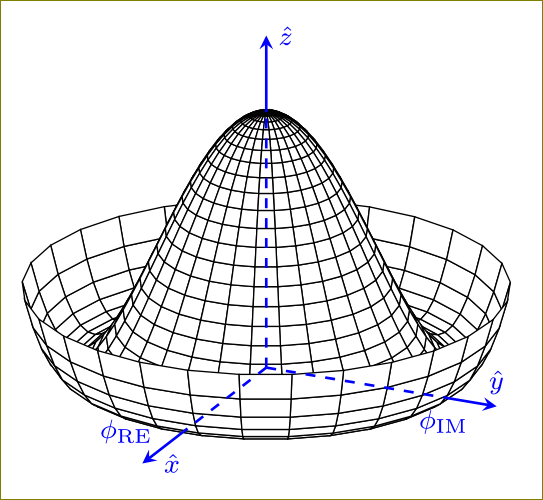
\includegraphics[width=0.4\linewidth]{figures/theory/higgs_potential.png}
    \caption{ A lower-dimensionality representation of the shape of the Higgs
potential.  The central peak represents a rotationally symmetric
unstable state, while the trough represents the infinite number of minima that
can be selected upon the spontaneous breaking of the symmetry.}
    \label{fig:higgs_potential}
  \end{center}
\end{figure}

The normed value of this minima can be calculated by taking the derivative of V
with respect to $\boldsymbol{\Phi}$ and setting it equal to $0$. This value,
also known as the vacuum expectation value (vev) has been found to be $v \equiv
\sqrt{-\mu^{2}/\lambda} = 246$ GeV. The arbitrary vev of the ground state Higgs
field is acquired when the symmetry of the Higgs potential is spontaneously
broken.  For ease of calculation the coordinate system is oriented such that

\begin{equation}
\left\langle \boldsymbol{\Phi}(x) \right\rangle = \frac{1}{\sqrt{2}} \left(
\begin{matrix} 0 \\ v \end{matrix} \right)
\end{equation} 

Next small perturbations around the minimum of the Higgs
potential are parametrized as 

\begin{equation} \label{eq:higgs:broken_higgs}
\left\langle \boldsymbol{\Phi}(x) \right\rangle = \frac{1}{\sqrt{2}} \left(
\begin{matrix} 0 \\ v + h(x) \end{matrix} \right) \text{exp} \left(
i\frac{\tau^{i}}{2}\theta^{i}(x) \right)
\end{equation} 

Here the real scalar field $h(x)$ corresponds to radial perturbations of the
minima, and the three $\theta^{i}(x)$ are the Nambu-Goldstone fields with
values determined by the choice of gauge.  Choosing the unitary gauge of
$\theta^{i}(x) = 0$ and expanding the kinetic term of
\Cref{eq:higgs:lagrangian} around the vev gives

\begin{equation} \label{eq:higgs:boson_masses}
\mathcal{L}_{\text{Higgs},K} = \frac{g^{2}v^{2}}{8} \left(
(W_{\mu}^{-})^{\dagger}W^{-\mu} + (W_{\mu}^{+})^{\dagger}W^{+\mu} \right) +
\frac{1}{2} \left( \begin{matrix} W_{\mu}^{3\dagger} & B_{\mu}^{\dagger}
\end{matrix} \right) \boldsymbol{M}^{2} \left( \begin{matrix} W^{3\mu} \\ B^{\mu}
\end{matrix} \right) + \ldots 
\end{equation}

Here the first term is the physical mass term for the $W^{\pm}$ bosons where
these charge eigenstates have been constructed out of the $W^{1,2}$ fields as
such $W^{\pm} = \frac{1}{\sqrt{2}}(W^{1} \mp iW^{2})$.  The second term
represents the mixture of the $W^{3}$ and $B$ fields through the mass matrix
$\boldsymbol{M}$.  Diagonalizing this matrix ($M_{D}$) and identifying the mass
eigenstates gives the physical fields of the photon ($\gamma$) and the $Z$
boson

\begin{equation}
\boldsymbol{M}_{D}^{2} = \left( \begin{matrix} 0 & 0 \\ 0 &
\frac{v^{2}}{4}(g_{W}^{2} + g^{'2)}   \end{matrix} \right)
\end{equation}

The upper left diagonal element corresponds to the massless photon
while the lower right diagonal element gives the mass of the massive $Z$ boson.
This results in the following masses for the four electroweak bosons

\begin{equation}
m_{W} = \frac{1}{2}g_{W}v \quad , \quad m_Z = \frac{1}{2}v\sqrt{g_{W}^{2} + g^{'2}}
\quad , \quad m_\gamma = 0
\end{equation}

The masses of the $W^{\pm}$ and $Z$ gauge bosons can be related through the
Weinberg mixing angle defined as

\begin{equation}
\theta_W = \cos^{-1}\left( \frac{g_{W}}{\sqrt{g_{W}^{2}+g^{'2}}} \right) \rightarrow m_{Z} =
\frac{m_{W}}{\cos{\theta_{W}}}
\end{equation}

Using this definition one can write out the exact mixture of $B$ and $W^{3}$ that
make up the photon and $Z$ boson as

\begin{align}
\gamma &= \text{cos}(\theta_{W})B + \text{sin}(\theta_{W})W^{3} \\
Z &= -\text{sin}(\theta_{W})B + \text{cos}(\theta_{W})W^{3}
\end{align}

\subsection{Fermion Mass Terms} \label{sec:theory:fermion_mass}

\Cref{sec:theory:gsw} shows how a simple fermion mass terms violate gauge
invariance due to the mixing of the left and right chiral states.  The Higgs
mechanism, however, allows for a gauge-invariant method of generating mass
terms through the Yukawa coupling of the Higgs field to the fermion fields.  An
example is the Yukawa coupling term for a quark doublet
($\boldsymbol{\Psi}_{L}$) and singlet ($\Psi_R$) coupling to the Higgs field
($\boldsymbol{\Phi}$) after spontaneous symmetry breaking, with the form
shown in \Cref{eq:higgs:broken_higgs}, when the unitary gauge $\Phi^{i}(x) = 0$
is chosen.
%
\begin{align}
\mathcal{L}_{\text{Yukawa}} &= - g_{b} \left[ \boldsymbol{\bar{\Psi}_L}
\boldsymbol{\Phi} \Psi_R + \bar{\Psi}_{R} \boldsymbol{\Phi}^{\dagger} \boldsymbol{\Psi_L}
\right] \\ &= - \frac{g_{b}}{\sqrt{2}} \left[ \left( \begin{matrix}
\bar{t} & \bar{b} \end{matrix} \right)_L \left( \begin{matrix} 0 \\ v +
h \end{matrix} \right) b_{R} + \bar{b}_{R} \left( \begin{matrix} 0 & (v + h)
\end{matrix} \right) \left( \begin{matrix} t \\ b \end{matrix} \right)_L \ \right] \\ &= - \underbrace{\frac{g_{b}}{\sqrt{2}}
v}_{m_{b}} \left( \bar{b}_{L}b_{R} + \bar{b}_{R}b_{L}  \right)
- \underbrace{\frac{g_{b}}{\sqrt{2}}}_{g_{b,h}} h \left(
\bar{b}_{L}b_{R} + \bar{b}_{R}b_{L}  \right) 
\end{align}
%
In this way mass terms are generated for the fermion field and the gauge
invariance of the Lagrangian is maintained via the proper combination of
covariant derivatives and fields.  This operation also produces the second term
which represents the coupling of the bottom quark to the Higgs itself and thus
gives the form of its coupling constant $g_{b,h}$.  Using this newly found
mass of the bottom quark $m_{b}$ the coupling can be written as
%
\begin{equation}
g_{b,h} = \frac{g_{b}}{\sqrt{2}} = \frac{m_{b}}{v}.
\end{equation}
%
Thus the coupling of the Higgs boson to a fermion is proportional
to the mass of the fermion itself. 
 
\subsection{The Higgs Boson}

It has been shown that the Higgs mechanism properly mixes the gauge fields to
provide the correct gauge-invariant mass terms, and also properly combines the
left and right chiral states of fermions to produce their mass terms.  During
spontaneous symmetry breaking of the electroweak potential three of the four
degrees of freedom in the Higgs doublet (\Cref{eq:higgs:higgs_field}) become
Goldstone bosons.  Since this theory is gauged these Goldstone bosons are
``eaten" by the 3 gauge bosons $W^{\pm}$ and $Z$ to form their longitudinal
components thus give them their mass.  However, the final broken degree of
freedom is absorbed by the new massive scalar particle, the Higgs boson
\cite{Higgs:1964pj}.

Focusing on the Higgs potential term (V) of
\Cref{eq:higgs:lagrangian} and substituting in the definition for
$\boldsymbol{\Phi}$ given in \Cref{eq:higgs:broken_higgs} gives
%
\begin{equation}
\mathcal{L}_\text{Higgs,V} = \frac{1}{2} \mu^{2} v^{2} - \mu^{2} h^{2} +
\lambda v h^{3} + \frac{1}{4} \lambda h^{4}
\end{equation}
%
The first term is constant and thus can be ignored.  The second term is the
mass term for the Higgs boson, $m_h = \sqrt{-2\mu^{2}} = \sqrt{2\lambda}v$.
Remembering that $h = h(x)$ was used for small radial perturbations of the
Higgs field the Higgs boson can be identified as a radial excitation of the
Higgs field.  Finally, the third and fourth terms represent the Higgs boson
self-couplings.  With these couplings and mass terms in hand the next step is
to experimentally verify this theory as discussed next in \Cref{chap:higgs}.

\section{Parton Distribution Function} \label{sec:theory:pdf}

Before QFT the proton was thought to be a hard ball containing no smaller
constituents.  However, we know now that that the strong field inside the proton
allows for any strong object to exist with some probability which changes based
off of the total energy of the proton.  This behavior is represented then by a
Probability Distribution Function.


